\chapter{Вплив просторового розташування кілець та механізми зміни рушійної сили}
\label{ch:ring-placement}

У попередньому розділі встановлено, що одночасна зміна жорсткості трьох кілець може змінювати енергетичну рушійну силу та напрямок приросту тріщини по-різному. Проте сумарний ефект не дає інформації про роль окремих неоднорідностей. Зокрема, екранування тріщини трьома жорсткими кільцями не означає екранування кожним кільцем. У цьому розділі спочатку розглянемо вибіркову активацію кільцевих областей, потім дослідимо поля напружень та енергії деформації. Метою є не лише встановлення ефективніших архітектур, а й пояснення різних знаків їхнього впливу.

\section{Вибіркова зміна матеріальних характеристик}
\label{sec:ring-design}

Розглянемо зафіксовану однорідну геометрію S2 ($s=33{,}4$ мм). Координати вершини приблизно $(103{,}409;33{,}192)$ мм, кут локальної дотичної з віссю $x$ становить $76{,}45^\circ$. Позначимо через $\mathcal S\subseteq\{1,2,3\}$ множину активних кілець. Для спільного множника модуля $\lambda$ задаємо
\begin{equation}
 E_k=E_{\mathrm m}\begin{cases}
 \lambda,&k\in\mathcal S,\\
 1,&k\notin\mathcal S .
 \end{cases}
 \label{eq:ring-mask}
\end{equation}
Для кожного з двох значень $\lambda=0{,}5$ та 2 розглядаємо всі вісім підмножин, включно з порожньою. Отже, маємо 16 логічних випадків та 15 різних розподілів матеріальних характеристик: порожня множина відповідає одному й тому самому однорідному розв'язку. Вихідні однорідна конфігурація та дві конфігурації з усіма активними кільцями відтворюють попередню серію побітово; додатково обчислено 12 задач з неповними множинами. Геометрія, навантаження та сітка в усіх цих порівняннях однакові.

\begin{table}[htbp]
 \centering
 \caption{Положення кілець відносно вершини S2}
 \label{tab:ring-positions}
 \begin{tabular}{rrrrr}
 \toprule
 Кільце & $x_1$, мм & $x_2$, мм & Відстань, мм & Кут, град\\
 \midrule
 1 & 47,112 & $-39,042$ & 61,187 & $-39,649$\\
 2 & 96,499 & $-27,144$ & 100,244 & $-15,711$\\
 3 & 145,886 & $-15,246$ & 146,681 & $-5,966$\\
 \bottomrule
 \end{tabular}
\end{table}

У табл.~\ref{tab:ring-positions} координати центрів подано у локальному базисі вершини, кут відраховано від дотичної. Усі три центри лежать на одному боці від локальної осі тріщини, проте відстані та кути істотно різні. Дискретна площа кожного кільця однакова і становить $1012{,}152529$ мм$^2$. Тому порівняння трьох одиночних кілець при однаковому $\lambda$ є контрольованим дослідженням розташування за однакової кількості зміненого матеріалу. Необхідно водночас враховувати, що відстань, кут та положення відносно опор і сили змінюються разом; ця серія не відокремлює вплив кожного геометричного параметра.

\section{Енергетичні та напрямні ефекти однакової активної площі}
\label{sec:ring-results}

Позначимо через $F_G(\mathcal S;\lambda)$ контраст~\eqref{eq:problem-fixed-contrast}, а через $F_\theta(\mathcal S;\lambda)=\theta(\mathcal S;\lambda)-\theta_{\mathrm H}$ різницю локальних кутів МКН. Обидві величини дорівнюють нулю для порожньої множини. Результати наведено в табл.~\ref{tab:ring-results}; усі значення є прямими матеріальними ефектами на одній геометрії, а не результатами поширення тріщини.

\begin{table}[htbp]
 \centering
 \caption{Ефекти вибіркової активації кілець на S2}
 \label{tab:ring-results}
 \begin{tabular}{lrrrr}
 \toprule
 & \multicolumn{2}{c}{$F_G$, \%} & \multicolumn{2}{c}{$F_\theta$, град}\\
 \cmidrule(lr){2-3}\cmidrule(lr){4-5}
 $\mathcal S$ & $\lambda=0{,}5$ & $\lambda=2$ & $\lambda=0{,}5$ & $\lambda=2$\\
 \midrule
 $\varnothing$ & 0 & 0 & 0 & 0\\
$\{1\}$ & $4,430$ & $-3,652$ & $1,311$ & $-1,110$ \\
$\{2\}$ & $-3,628$ & $3,035$ & $-0,371$ & $0,306$ \\
$\{3\}$ & $2,331$ & $-1,825$ & $-0,353$ & $0,288$ \\
$\{1,2\}$ & $0,316$ & $-0,906$ & $1,058$ & $-0,734$ \\
$\{1,3\}$ & $6,747$ & $-5,478$ & $0,984$ & $-0,806$ \\
$\{2,3\}$ & $-1,675$ & $0,980$ & $-0,767$ & $0,574$ \\
$\{1,2,3\}$ & $2,181$ & $-2,931$ & $0,694$ & $-0,452$ \\
 \bottomrule
 \end{tabular}
\end{table}

\begin{figure}[htbp]
 \centering
 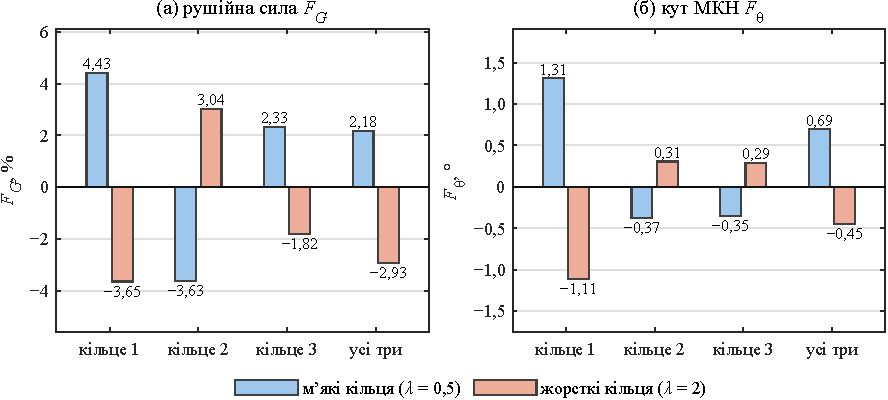
\includegraphics[width=\textwidth]{figures/F06_1_vnesky_kilets.pdf}
 \caption{Енергетичні та напрямні ефекти окремих кілець і одночасної активації всіх трьох кілець на фіксованій геометрії S2.}
 \label{fig:ring-single}
\end{figure}

Перший важливий результат полягає в тому, що кільце 2 впливає на $G$ протилежно до кілець 1 і 3. Пом'якшення кільця 1 збільшує $G$ на 4,43\,\%, тоді як пом'якшення кільця 2 зменшує його на 3,63\,\%. Різниця становить 8,06 відсоткового пункта за однакових модулів і активної площі. Ця різниця розрізняється за обома прийнятими критеріями. Вплив третього кільця за модулем менший, проте його знак збігається зі знаком першого. Для жорстких кілець знаки всіх трьох ефектів протилежні відповідним ефектам м'яких кілець. Водночас за консервативним критерієм енергетичні ефекти жорсткого кільця 2 та третього кільця при обох контрастах залишаються нерозрізненими.

Віддаленість сама по собі не визначає знака ефекту. За модулем одиночні енергетичні ефекти в цій серії справді впорядковуються відповідно до відстані: $|F_G(\{1\})|>|F_G(\{2\})|>|F_G(\{3\})|$. Проте навіть третє кільце, центр якого віддалений приблизно на 147 мм, дає обчислений контраст порядку двох відсотків. Залежність знака від розташування є істотною особливістю задачі, яка не випливає з простої оцінки затухання локального збурення біля тріщини.

Для кута МКН інша група знаків: кільце 1 має протилежний напрямний ефект до кілець 2 і 3. Найближче кільце змінює кут у 3,5--3,9 раза сильніше, ніж кожне з двох інших. Таким чином, групування кілець за знаком енергетичного ефекту не збігається з групуванням за знаком напрямного. Це узгоджується з розмежуванням модових чутливостей у підрозділі~\ref{sec:fixed-steering}.

\begin{figure}[htbp]
 \centering
 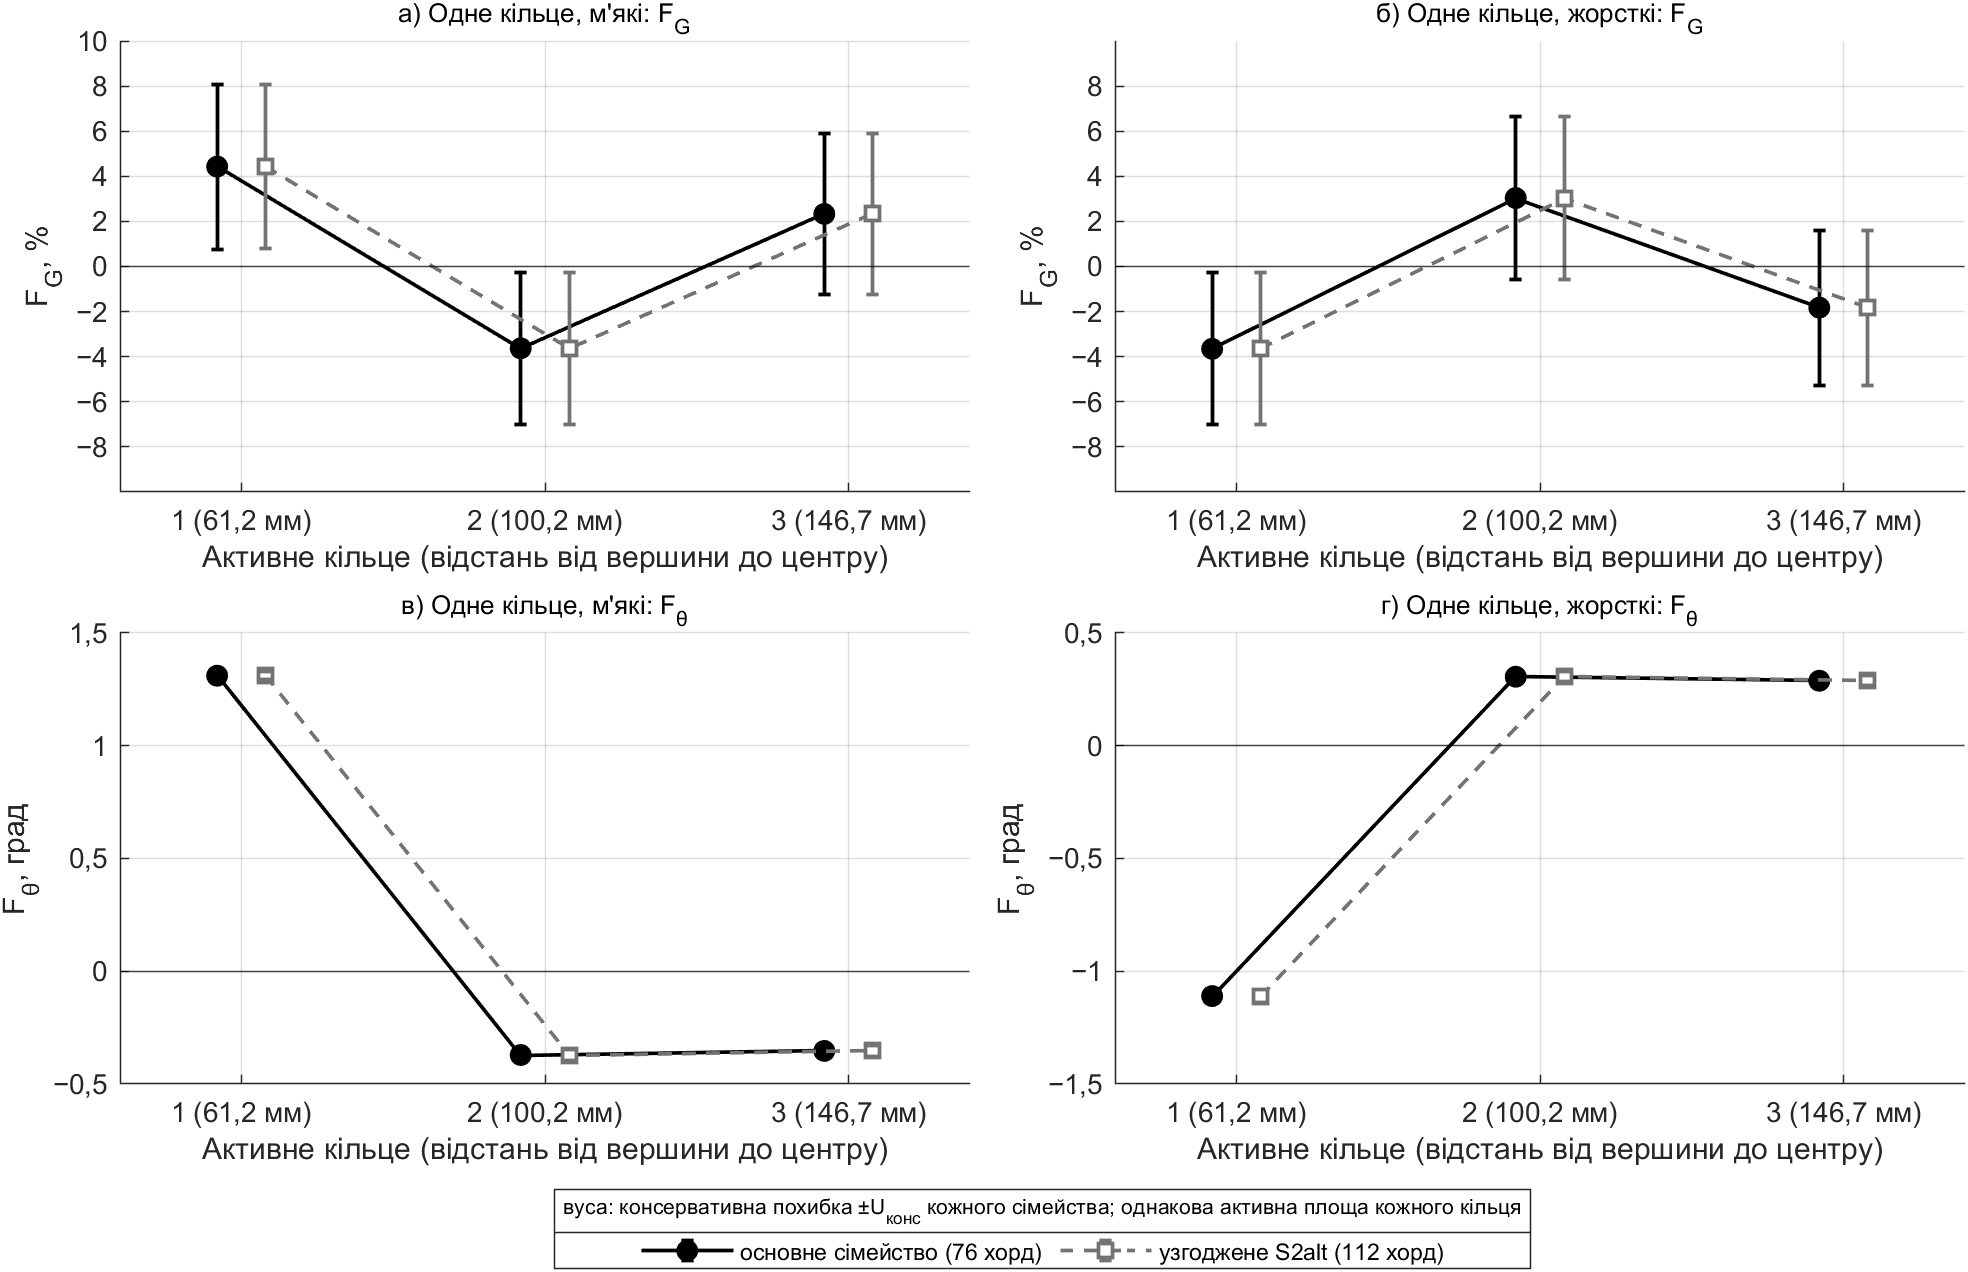
\includegraphics[width=\textwidth]{figures/r1_g3_equal_area_grey.png}
 \caption{Ефекти одиночних кілець при однаковій активній площі: порівняння вихідної та альтернативної зовнішніх сіток на S2.}
 \label{fig:ring-equal-area}
\end{figure}

Порівняння R1 підтвердило стійкість усіх шести одиночних енергетичних і шести кутових контрастів до конкретної заміни зовнішньої сітки. Збережено також усі чотири порядки ранжування (два контрасти жорсткості та дві характеристики). Детальні чисельні показники наведено в підрозділі~\ref{sec:ver-exterior}. Не слід переносити це приймання на всі комбінації: на альтернативній сітці з двокільцевих варіантів розглянуто лише жорстку пару $\{1,3\}$.

Друга важлива закономірність стосується комбінацій. За однакової площі двох жорстких кілець контрасти для $\{1,2\}$, $\{1,3\}$ та $\{2,3\}$ становлять відповідно $-0{,}906$, $-5{,}478$ та $+0{,}980$\,\%. Отже, збільшення кількості жорсткого матеріалу не гарантує зменшення $G$. Найменше $G$ серед розглянутих конфігурацій отримано для жорсткої пари $\{1,3\}$, а найбільше --- для м'якої пари $\{1,3\}$. Це не глобальна оптимізація: не змінювалися радіуси, координати кілець, змішані контрасти або схема навантаження.

\begin{figure}[htbp]
 \centering
 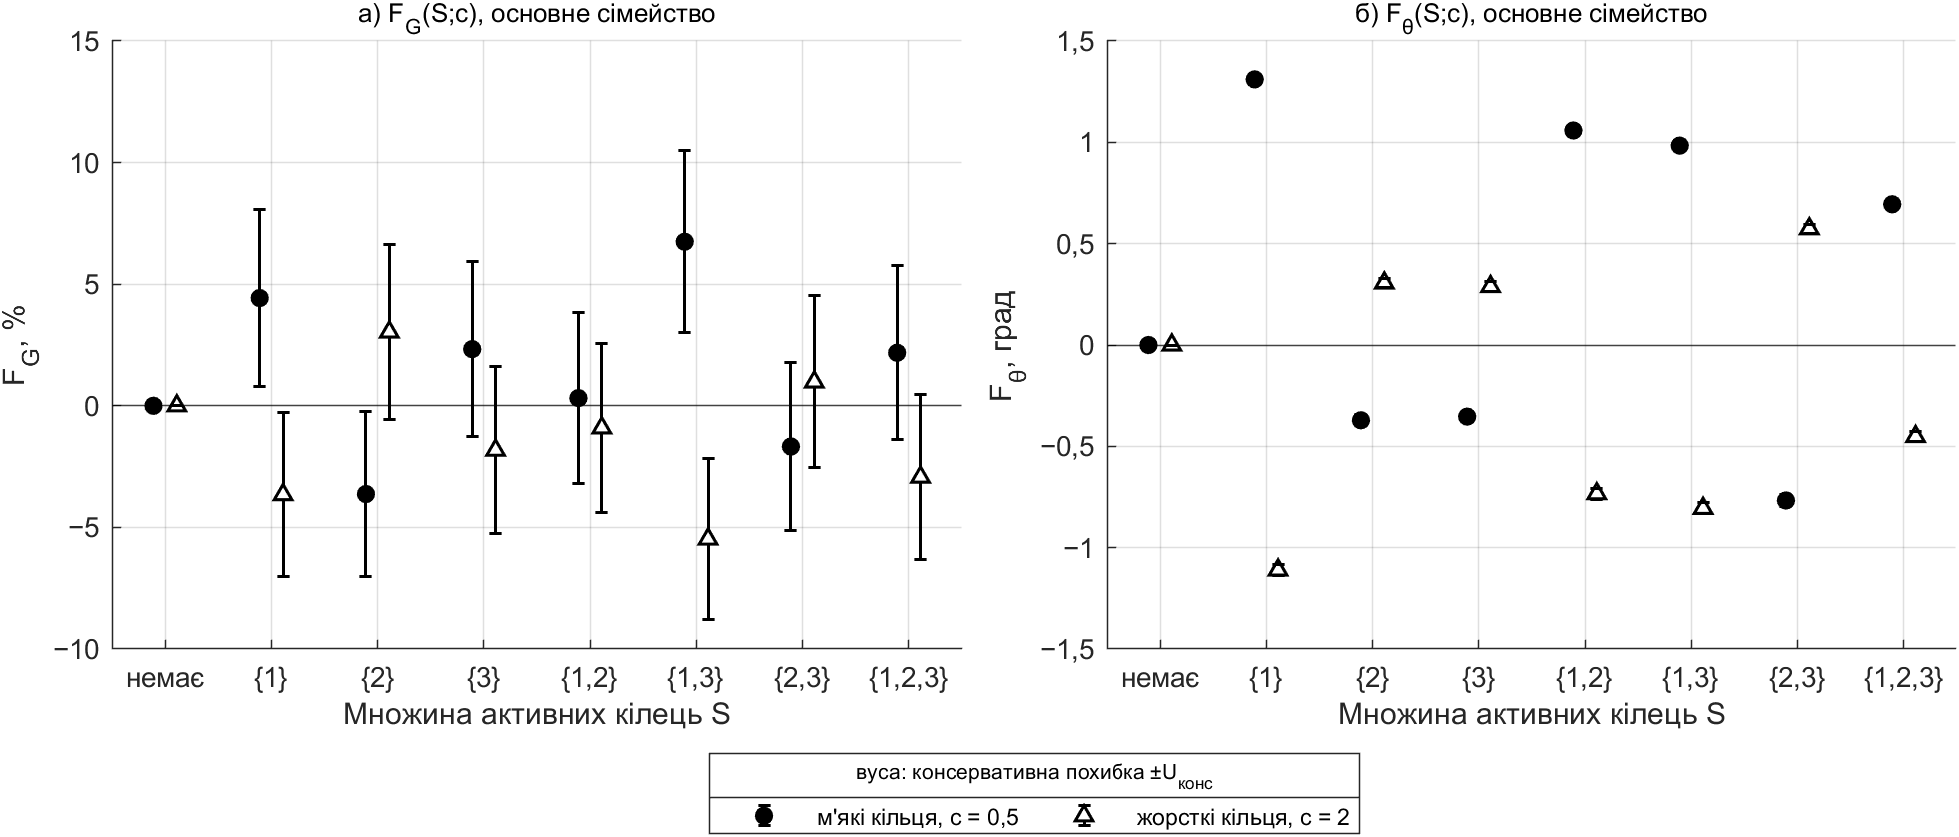
\includegraphics[width=\textwidth]{figures/r1_g6_m4b_masks_grey.png}
 \caption{Енергетичні й напрямні характеристики конфігурацій з різними множинами активних кілець на вихідній сітці S2.}
 \label{fig:ring-masks}
\end{figure}

\section{Адитивність і взаємодія матеріальних неоднорідностей}
\label{sec:ring-nonadditive}

Чи можна оцінити сумарний вплив декількох кілець, підсумовуючи ефекти одиночних? Для довільної характеристики $F$ (далі $F_G$ або $F_\theta$) і фіксованого контрасту $\lambda$ введемо
\begin{equation}
 f_i=F(\{i\}),\qquad
 I_{ij}=F(\{i,j\})-f_i-f_j.
 \label{eq:ring-pair}
\end{equation}
Внесок потрійної взаємодії визначимо як
\begin{equation}
 I_{123}=F(\{1,2,3\})-\sum_i f_i-\sum_{i<j}I_{ij}.
 \label{eq:ring-triple}
\end{equation}
Тоді точна тотожність
\begin{equation}
 F(\{1,2,3\})=\sum_i f_i+\sum_{i<j}I_{ij}+I_{123}
 \label{eq:ring-reconstruct}
\end{equation}
є розкладом функції множини за включенням і виключенням. Він не передбачає фізичної лінійності щодо контрасту жорсткості. Зокрема, лінійність крайової задачі за навантаженням не означає лінійності розв'язку за матрицею жорсткості. Крім того, $G$ є квадратичною, а кут МКН --- нелінійною функцією КІН. Ненульові $I$ можуть відображати обидві ці обставини; без додаткового розкладу їх не можна ототожнювати тільки з просторовою взаємодією полів.

Для симетричного розподілу сумарного ефекту між окремими кільцями використовуємо також величини Шеплі:
\begin{equation}
 \phi_i=f_i+\frac12\sum_{j\ne i}I_{ij}+\frac13 I_{123},
 \qquad \sum_i\phi_i=F(\{1,2,3\}).
 \label{eq:ring-shapley}
\end{equation}
Це середній граничний внесок кільця при всіх порядках його додавання. Величини $\phi_i$ не є незалежними фізичними енергіями і відрізняються від ефектів одиночних кілець.

\begin{table}[htbp]
 \centering
 \caption{Розклад енергетичних і кутових контрастів на S2. Зірочка означає розрізнення за обома критеріями; інші наведені внески розрізняються лише за первинним.}
 \label{tab:ring-decomp}
 \begin{tabular}{lrrrr}
 \toprule
 & \multicolumn{2}{c}{$F_G$, \%} & \multicolumn{2}{c}{$F_\theta$, град}\\
 \cmidrule(lr){2-3}\cmidrule(lr){4-5}
 Внесок & $\lambda=0{,}5$ & $\lambda=2$ & $\lambda=0{,}5$ & $\lambda=2$\\
 \midrule
$f_{1}$ & $4,4298^{*}$ & $-3,6517^{*}$ & $1,3106^{*}$ & $-1,1100^{*}$ \\
$f_{2}$ & $-3,6278^{*}$ & $3,0352$ & $-0,3714^{*}$ & $0,3061^{*}$ \\
$f_{3}$ & $2,3310$ & $-1,8248$ & $-0,3534^{*}$ & $0,2883^{*}$ \\
$I_{12}$ & $-0,4861$ & $-0,2893$ & $0,1192^{*}$ & $0,0703^{*}$ \\
$I_{13}$ & $-0,0143$ & $-0,0014$ & $0,0264$ & $0,0158$ \\
$I_{23}$ & $-0,3780$ & $-0,2301$ & $-0,0424$ & $-0,0207$ \\
$I_{123}$ & $-0,0733$ & $0,0309$ & $0,0054$ & $-0,0014$ \\
$\phi_{1}$ & $4,1552^{*}$ & $-3,7868^{*}$ & $1,3852^{*}$ & $-1,0674^{*}$ \\
$\phi_{2}$ & $-4,0843^{*}$ & $2,7858$ & $-0,3313^{*}$ & $0,3304^{*}$ \\
$\phi_{3}$ & $2,1105$ & $-1,9303$ & $-0,3596^{*}$ & $0,2854^{*}$ \\
 \bottomrule
 \end{tabular}
\end{table}

\begin{figure}[htbp]
 \centering
 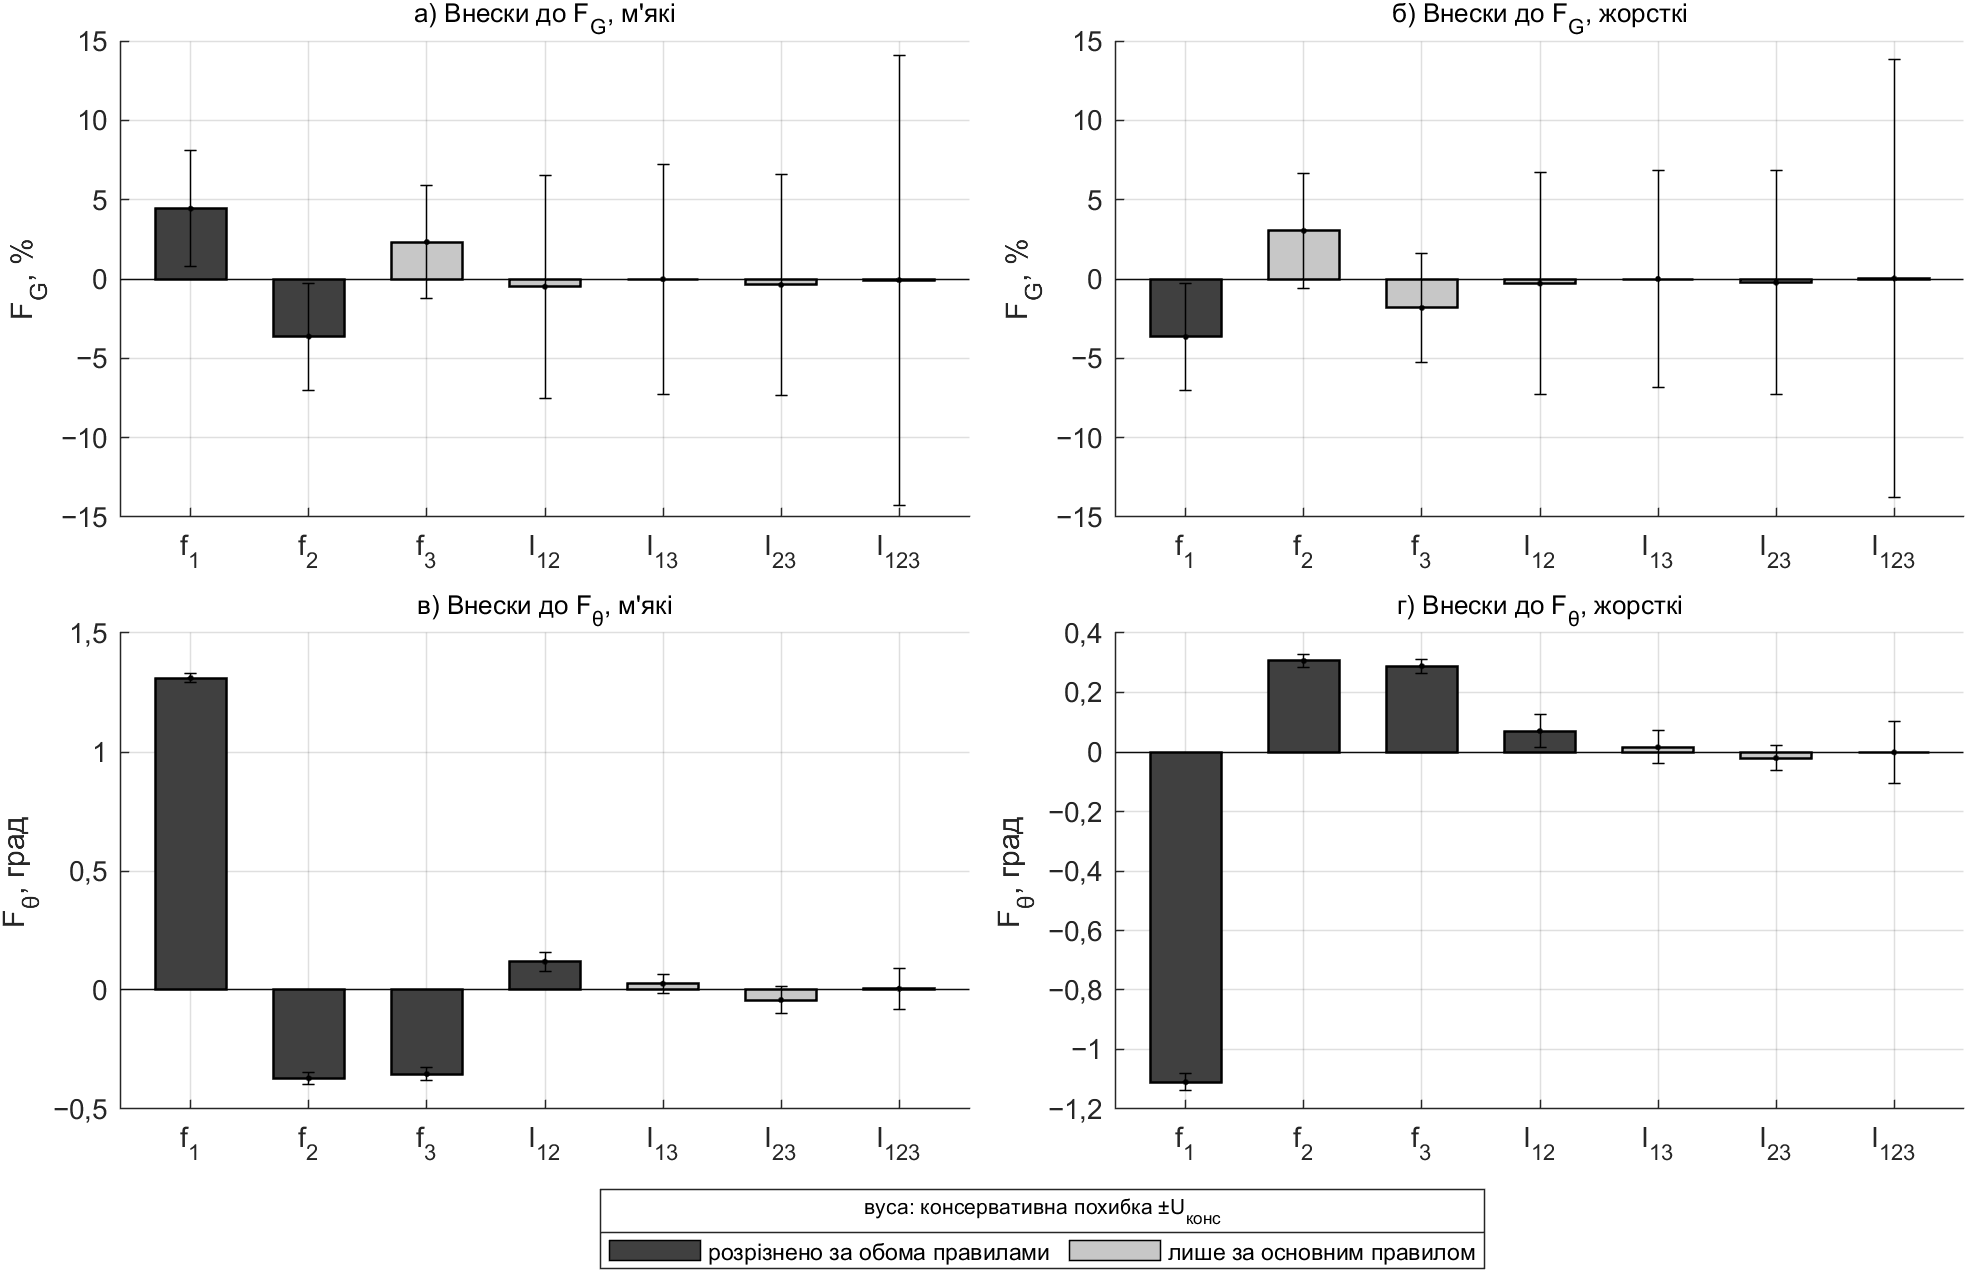
\includegraphics[width=\textwidth]{figures/r1_g7_m4b_decomposition_grey.png}
 \caption{Основні внески та взаємодії матеріальних неоднорідностей; розрізнення за первинним і консервативним критеріями.}
 \label{fig:ring-decomp}
\end{figure}

Для трьох м'яких кілець сума одиночних ефектів становить приблизно $+3{,}133$\,\%, а сумарний ефект --- $+2{,}181$\,\%. Різниця близько $-0{,}952$ відсоткового пункта складається з усіх взаємодій. Для жорстких кілець відповідні величини $-2{,}441$ та $-2{,}931$\,\%. Найбільші парні енергетичні взаємодії за модулем не перевищують 0,49 відсоткового пункта; вони менші за основні ефекти, але можуть бути істотними при взаємному компенсуванні останніх.

Усі енергетичні взаємодії розрізняються за первинним критерієм, однак жодна --- за консервативним. Особливо мала взаємодія $I_{13}$ для жорстких кілець (близько $-1{,}44\cdot10^{-5}$ у безрозмірних одиницях) має порядок спостереженої міжсіткової зміни одиночних контрастів. Не слід приписувати її знаку фізичний зміст. Незалежне повторення всього розкладу на іншій сітці не виконано. Для кута МКН взаємодія $I_{12}$ розрізняється за обома критеріями при обох контрастах; інші взаємодії --- лише за первинним.

Таким чином, просте підсумовування одиночних внесків є наближенням, а не точною властивістю матеріальної архітектури. Вибір конфігурацій для подальшого дослідження має враховувати не тільки знак одиночного ефекту, а й можливе компенсування внесків.

\section{Поля напружень та енергії деформації}
\label{sec:ring-fields}

Для пояснення результатів відновлено напруження, деформації та густину енергії
\begin{equation}
 w(\boldsymbol x)=\tfrac12\boldsymbol\sigma(\boldsymbol x):
 \boldsymbol\varepsilon(\boldsymbol x)
 \label{eq:ring-w}
\end{equation}
зі збережених переміщень T6 для однорідного стану та шести одиночних кілець на двох сітках. Енергії елементів, обчислені триточковою квадратурою, збігаються зі збереженими до $1{,}9\cdot10^{-13}$ у відносних одиницях. Це перевірка відтворення поля, а не експериментальна валідація.

\begin{figure}[htbp]
 \centering
 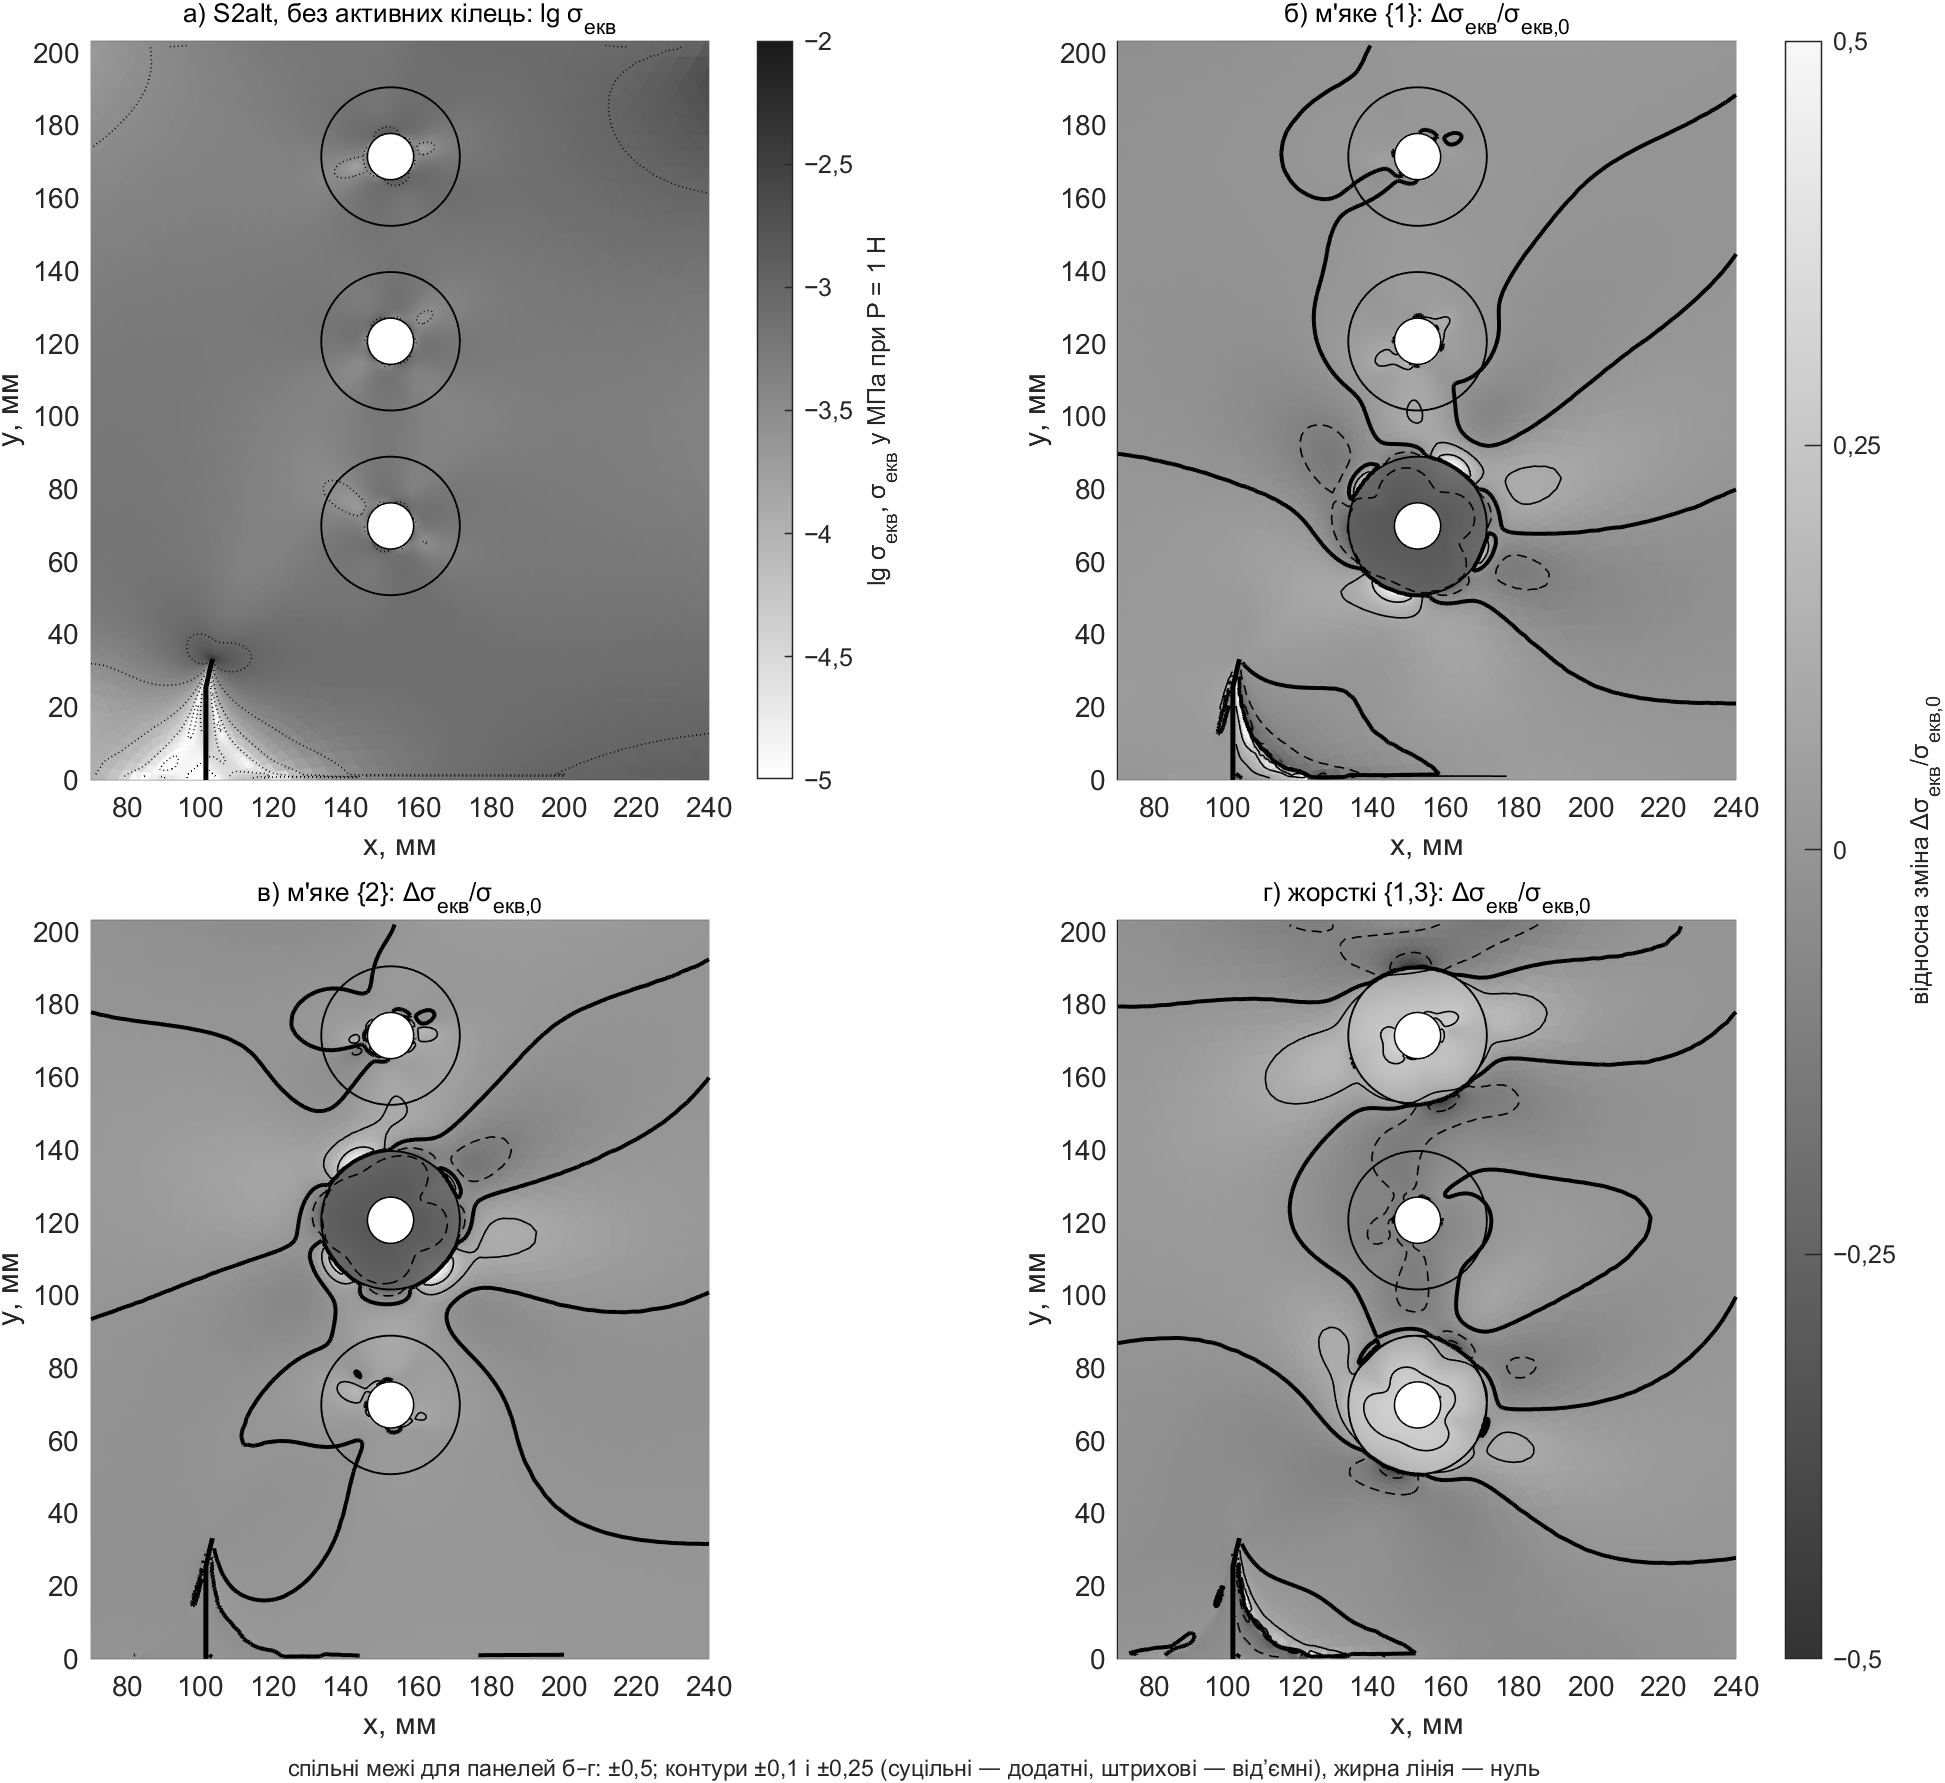
\includegraphics[width=\textwidth]{figures/r1_g4_stress_global_grey.png}
 \caption{Еквівалентні напруження однорідної пластини та відносна зміна поля для вибраних архітектур на альтернативній сітці S2. Для відносних змін використано спільну шкалу.}
 \label{fig:ring-von-mises}
\end{figure}

\begin{figure}[htbp]
 \centering
 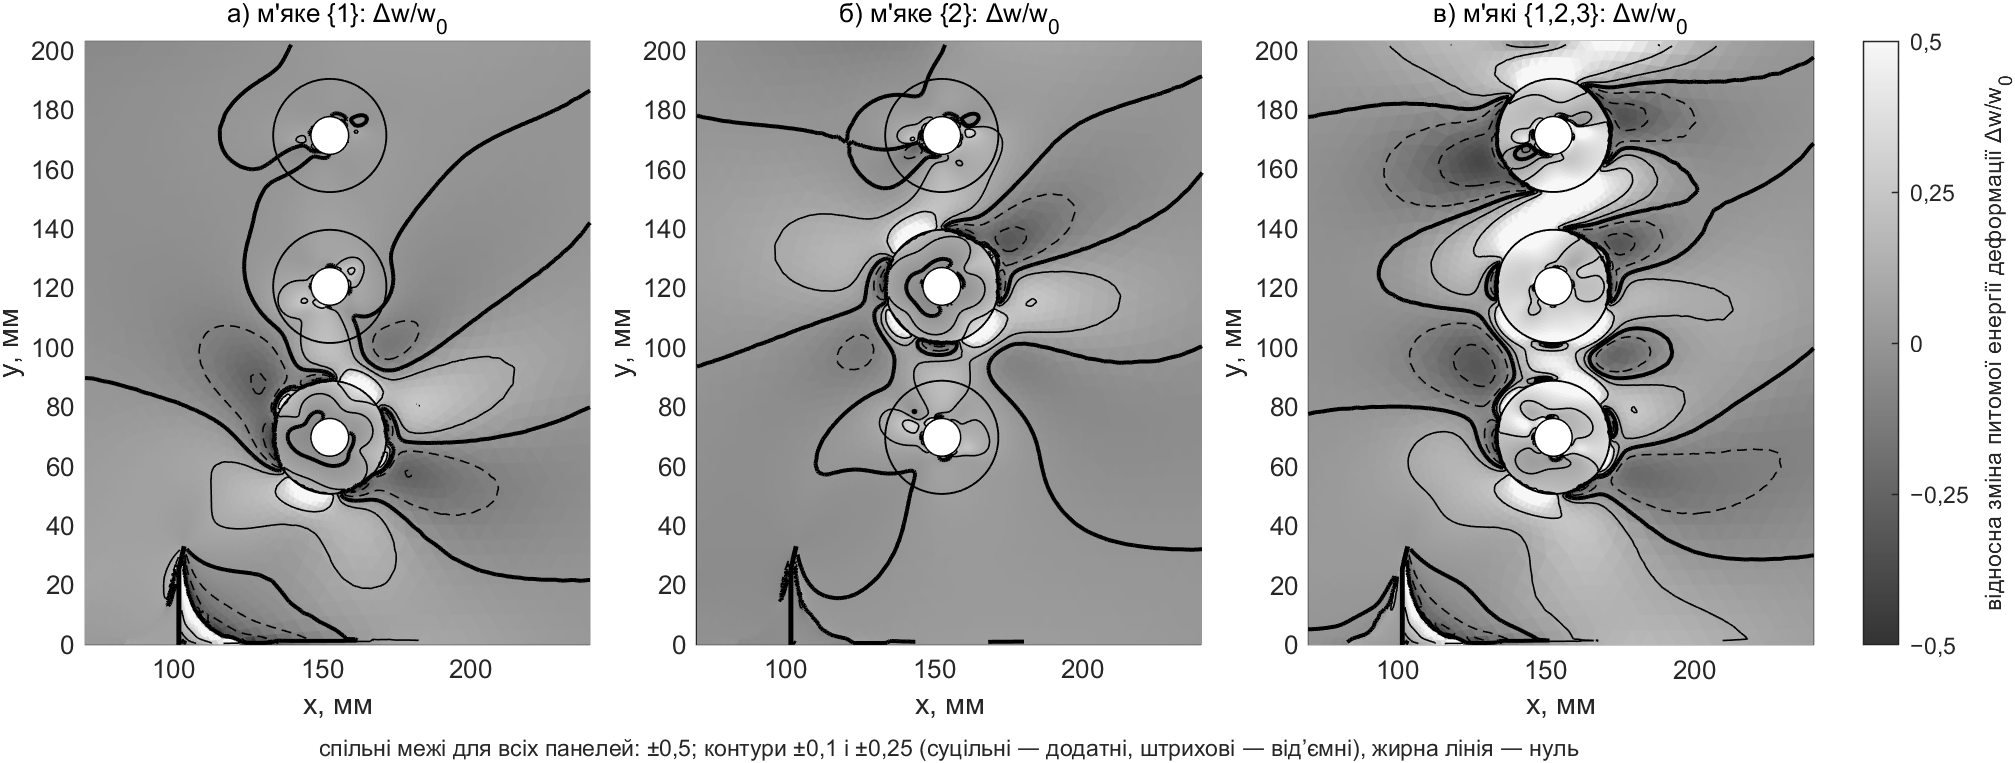
\includegraphics[width=\textwidth]{figures/r1_g5_energy_density_grey.png}
 \caption{Відносна зміна середньої по елементах густини енергії деформації для вибраних м'яких кілець на вихідній сітці S2; спільна шкала відносних змін.}
 \label{fig:ring-energy-maps}
\end{figure}

Карти еквівалентного напруження показують, що м'які кільця зменшують напруження в активованих областях, тоді як жорсткі збільшують їх. Для розглянутих м'яких кілець медіанне зменшення еквівалентного напруження в активній області становить близько 29\,\%; для жорсткої пари зростання в кільцях 1 і 3 становить приблизно 26 та 22\,\%. При цьому медіанна зміна в матриці мала, але просторове збурення простежується далеко від активної області. Карти енергії (рис.~\ref{fig:ring-energy-maps}) також показують перерозподіл по навантаженій частині пластини. Ці відомості не встановлюють знак зміни $G$: для цього потрібно дослідити зміну поля при варіації геометрії тріщини.

\subsection{Гіпотеза про передачу навантаження від сили до опори}

Пряма між лівою опорою та точкою прикладання сили проходить на відстані 5,8 мм від центра кільця 2. Центри кілець 1 і 3 розташовані по різні боки від неї (відповідні знакові відстані $-32{,}2$ та $+43{,}8$ мм). Виникає гіпотеза, що кільце 2 належить до особливої області передачі навантаження і тому його вплив протилежний впливу двох інших кілець. Перевіримо, чи є ця пряма траєкторією головного стиску або областю концентрації енергії.

\begin{figure}[htbp]
 \centering
 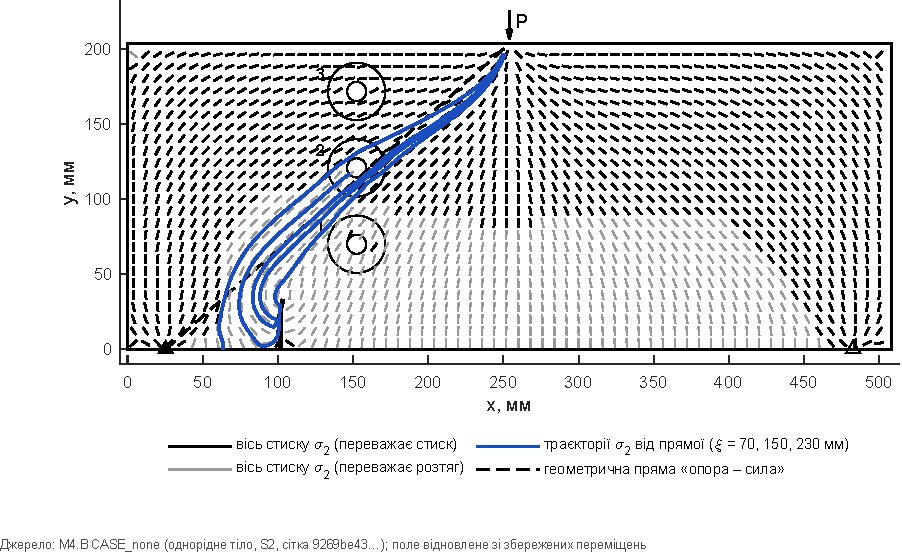
\includegraphics[width=\textwidth]{figures/G1_1_napriamy_stysku_UA.pdf}
 \caption{Осі меншого головного напруження та наближені траєкторії цих осей у однорідній пластині S2. Пряму між лівою опорою і силою використано як геометричний орієнтир.}
 \label{fig:ring-principal}
\end{figure}

\begin{figure}[htbp]
 \centering
 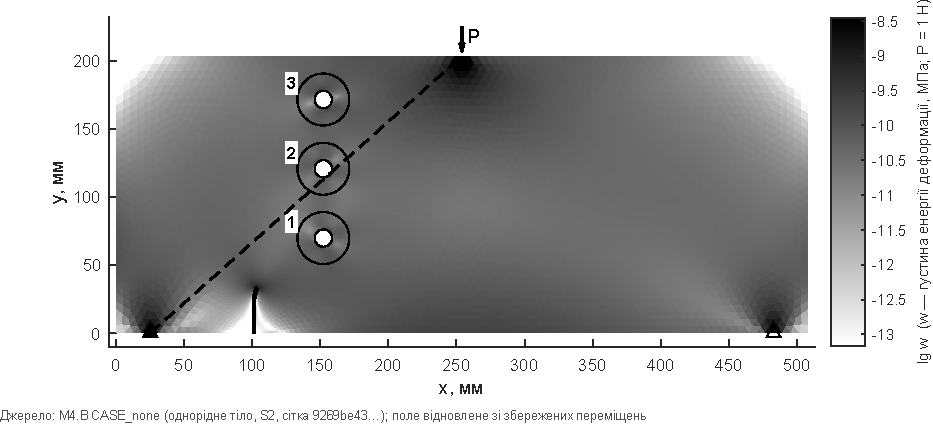
\includegraphics[width=\textwidth]{figures/G1_2_gustyna_energii_UA.pdf}
 \caption{Густина енергії деформації однорідної пластини S2 (логарифмічна шкала, сила 1 Н). Поле відновлено зі збережених переміщень.}
 \label{fig:ring-w-reference}
\end{figure}

У смузі півшириною 10 мм навколо прямої медіанне відхилення осі стиску від напряму прямої дорівнює $11{,}4^\circ$; приблизно 61\,\% площі має відхилення не більше $15^\circ$. У двох паралельних смугах зі зміщеннями $\pm30$ мм відповідні медіанні кути становлять $16{,}1^\circ$ та $14{,}8^\circ$. Уздовж верхньої частини прямої траєкторії осей стиску відхиляються від неї не більше ніж приблизно на 10 мм; нижче отвору 2 відхилення досягають 26--44 мм, і жодна з досліджених ліній не досягає лівої опори. Ці лінії відновлено чисельно з центроїдних напрямків елементів, тому вони є наближеними траєкторіями, а не точними характеристиками неперервного поля.

Області найбільших стискальних напружень не збігаються з прямою. У кількох поперечних перерізах їхні екстремуми розташовані на 38--52 мм вище неї. Середні густини енергії в центральній та зміщеній на 30 мм смугах майже однакові ($5{,}63\cdot10^{-11}$ та $5{,}69\cdot10^{-11}$ МПа). Таким чином, пряму не можна вважати ні повною траєкторією головних напружень, ні гребенем стиску чи енергії.

\begin{table}[htbp]
 \centering
 \caption{Напружений стан областей кілець в однорідній пластині S2. Головні напруження усередненого тензора наведено в одиницях $10^{-4}$ МПа при $P=1$ Н.}
 \label{tab:ring-stress}
 \begin{tabular}{rrrrrr}
 \toprule
 Кільце & Відстань, мм & $\sigma_1$ & $\sigma_2$ & Кут, град & Стиск, \%\\
 \midrule
 1 & $-32,2$ & $+4,24$ & $-1,59$ & 21,1 & 12\\
 2 & $+5,8$ & $+1,92$ & $-3,81$ & 5,1 & 75\\
 3 & $+43,8$ & $+0,50$ & $-5,72$ & 27,1 & 96\\
 \bottomrule
 \end{tabular}
\end{table}

У табл.~\ref{tab:ring-stress} наведено власні значення усередненого по кільцю тензора, кут його осі стиску відносно прямої та частку площі, на якій стиск домінує за модулем головних напружень. Ця частка не є часткою двовісно стиснутого матеріалу. Зокрема, для кільця 2 $\sigma_1>0$, а $\sigma_2<0$; отже, усереднений стан має одночасно розтягальне та стискальне головні напруження з переважанням стиску. У кільці 1 переважає розтяг, у кільці 3 --- стиск. Попри це, кільця 1 і 3 мають однакові знаки енергетичних ефектів. Сам тип напруженого стану не визначає знак впливу на $G$.

\begin{figure}[htbp]
 \centering
 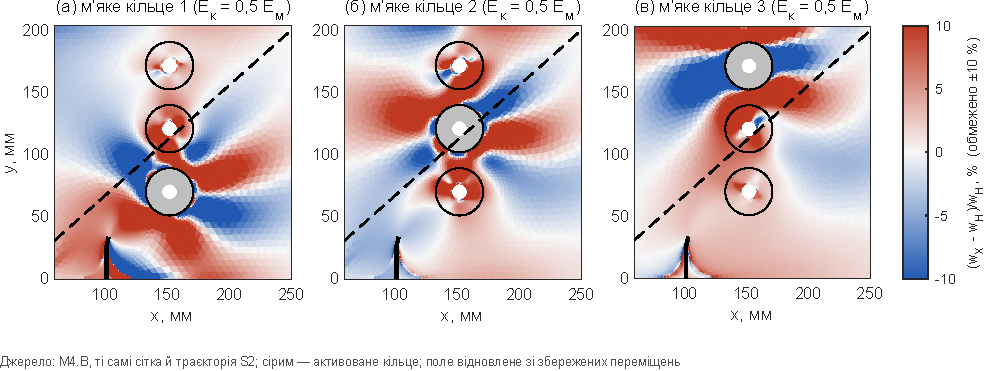
\includegraphics[width=\textwidth]{figures/G1_3_pererozpodil_energii_UA.pdf}
 \caption{Відносна зміна густини енергії поза активованим м'яким кільцем: (а) кільце 1, (б) кільце 2, (в) кільце 3. Активну область замасковано; шкала обмежена інтервалом від $-10$ до $+10$ відсотків.}
 \label{fig:ring-single-fields}
\end{figure}

Активація м'яких кілець створює області зменшення та збільшення густини енергії поза самими кільцями (рис.~\ref{fig:ring-single-fields}). Для кільця 2 область зменшення витягнута приблизно вздовж прямої опора--сила. Для інших кілець її орієнтація відрізняється. Проте просторовий розподіл $w_X-w_{\mathrm H}$ при фіксованій тріщині не є сам по собі полем чутливості $G$ до матеріального контрасту.

\section{Енергетична чутливість до локальної зміни матеріалу}
\label{sec:ring-sensitivity}

\subsection{Варіаційне обґрунтування}

Розглянемо фіксовану геометрію, лінійно-пружну систему під заданим навантаженням $P$. Нехай $\boldsymbol S$ --- тензор пружної податливості матеріалу, а $\boldsymbol S_{\mathrm H}$ --- його значення в однорідній матриці. За однакового коефіцієнта Пуассона зміна модуля в кільці $k$ еквівалентна
\begin{equation}
 \boldsymbol S_X-\boldsymbol S_{\mathrm H}
 =\eta_k\boldsymbol S_{\mathrm H},\qquad
 \eta_k=\lambda_k^{-1}-1,\quad \boldsymbol x\in\Omega_k .
 \label{eq:ring-eta}
\end{equation}
Поза активними кільцями ця різниця нульова. Для двох рівноважних полів на тій самій геометрії та при тих самих силах принцип віртуальних робіт дає
\begin{equation}
 \begin{aligned}
 P^2 C_X &=t\int_\Omega \boldsymbol\sigma_{\mathrm H}:
                     \boldsymbol\varepsilon_X\,\mathrm d\Omega,\\
 P^2 C_{\mathrm H}&=t\int_\Omega \boldsymbol\sigma_X:
                     \boldsymbol\varepsilon_{\mathrm H}\,\mathrm d\Omega .
 \end{aligned}
 \label{eq:ring-betti-works}
\end{equation}
Використовуючи симетрію тензорів податливості, отримаємо точну перехресну тотожність
\begin{equation}
 C_X-C_{\mathrm H}=\frac{t}{P^2}\sum_k\eta_k
 \int_{\Omega_k}
 \boldsymbol\sigma_{\mathrm H}:\boldsymbol S_{\mathrm H}:
 \boldsymbol\sigma_X\,\mathrm d\Omega .
 \label{eq:ring-betti}
\end{equation}
Вона справедлива також для дискретних полів на спільній узгодженій сітці при точному збиранні білінійних форм. Для 12 одиночних випадків (дві сітки) перехресний інтеграл відтворив записану зміну податливості; максимальна повідомлена розбіжність не перевищує $1{,}9\cdot10^{-10}$ за показником вихідного аудиту.

За малого контрасту та регулярної залежності розв'язку від матеріальних параметрів $\boldsymbol\sigma_X=\boldsymbol\sigma_{\mathrm H}+O(\|\boldsymbol\eta\|)$ у відповідній енергетичній нормі. Позначимо енергію однорідного тіла в області $k$ та повну енергію, віднесені до одиниці товщини, через
\begin{equation}
 \mathcal W_k^{\mathrm H}=\int_{\Omega_k} w_{\mathrm H}\,\mathrm d\Omega,
 \qquad \mathcal W_{\mathrm H}=\int_\Omega w_{\mathrm H}\,\mathrm d\Omega .
 \label{eq:ring-energies}
\end{equation}
Повна енергія дорівнює $t\mathcal W=P^2 C/2$. Із~\eqref{eq:ring-betti} випливає
\begin{equation}
 \mathcal W_X-\mathcal W_{\mathrm H}
 =\sum_k\eta_k\mathcal W_k^{\mathrm H}
 +O(\|\boldsymbol\eta\|^2).
 \label{eq:ring-first-energy}
\end{equation}
Це також є наслідком стаціонарності доповнювальної енергії: в першому порядку для варіації податливості достатньо однорідного поля. Розклад стосується енергії всієї конструкції, а не припущення про незмінність напружень у кільці за скінченного контрасту.

Якщо похідну за довжиною $s$ розуміти як похідну форми при одному й тому самому віртуальному прирості тріщини, то за силового навантаження $G=\partial_s\mathcal W$ (див.~\eqref{eq:fixed-compliance-G}). За достатньої гладкості змішаної чутливості з~\eqref{eq:ring-first-energy} отримуємо
\begin{equation}
 \left.\frac{\partial G}{\partial\eta_k}\right|_{\boldsymbol\eta=0}
 =\partial_s\mathcal W_k^{\mathrm H},
 \qquad
 F_G^{(1)}=\sum_k\eta_k
 \frac{\partial_s\mathcal W_k^{\mathrm H}}{\partial_s\mathcal W_{\mathrm H}}.
 \label{eq:ring-first-G}
\end{equation}
Отже, знак першого порядку визначає не сама густина енергії і не знак головного напруження, а похідна енергії в області майбутньої неоднорідності за геометричним приростом тріщини. Якщо ця область розвантажується при рості тріщини, то її пом'якшення у першому порядку зменшує $G$. Якщо довантажується, пом'якшення збільшує $G$.

Слід розрізняти точну похідну форми та її чисельне наближення різницями енергій уздовж ламаної однорідної траєкторії. В останньому випадку змінюються сітка і напрямок приросту, а точкове навантаження створює додаткову сіткову залежність енергії. Тому далі перевіряємо саме наближення~\eqref{eq:ring-first-G}, а не точну похідну форми. Для скінченних контрастів $\eta=1$ та $-0{,}5$ немає підстав вважати члени вищих порядків малими без додаткового дослідження.

\subsection{Зміна енергії в областях кілець уздовж однорідної траєкторії}

Використаємо збережені однорідні стани S0--S4. На цьому етапі матеріал усіх кілець збігається з матрицею, а їхні контури визначають області інтегрування. Енергії наведено в табл.~\ref{tab:ring-energies}. Відносні зміни в кільцях на порядок більші за відносну зміну повної енергії.

\begin{table}[htbp]
 \centering
 \caption{Енергії на одиницю товщини, Н: $\mathcal W_k$ в одиницях $10^{-8}$ Н; $\mathcal W_{\mathrm H}$ в одиницях $10^{-6}$ Н.}
 \label{tab:ring-energies}
 \begin{tabular}{lrrrr}
 \toprule
 Стан & $\mathcal W_1$ & $\mathcal W_2$ & $\mathcal W_3$ & $\mathcal W_{\mathrm H}$\\
 \midrule
 S0 & 4,499 & 4,857 & 6,412 & 8,650\\
 S1 & 4,646 & 4,647 & 6,521 & 8,687\\
 S2 & 4,876 & 4,422 & 6,653 & 8,732\\
 S3 & 5,213 & 4,183 & 6,812 & 8,783\\
 S4 & 5,684 & 3,935 & 7,001 & 8,841\\
 \midrule
 Зміна S0--S4, \% & $+26,3$ & $-19,0$ & $+9,2$ & $+2,2$\\
 \bottomrule
 \end{tabular}
\end{table}

\begin{figure}[htbp]
 \centering
 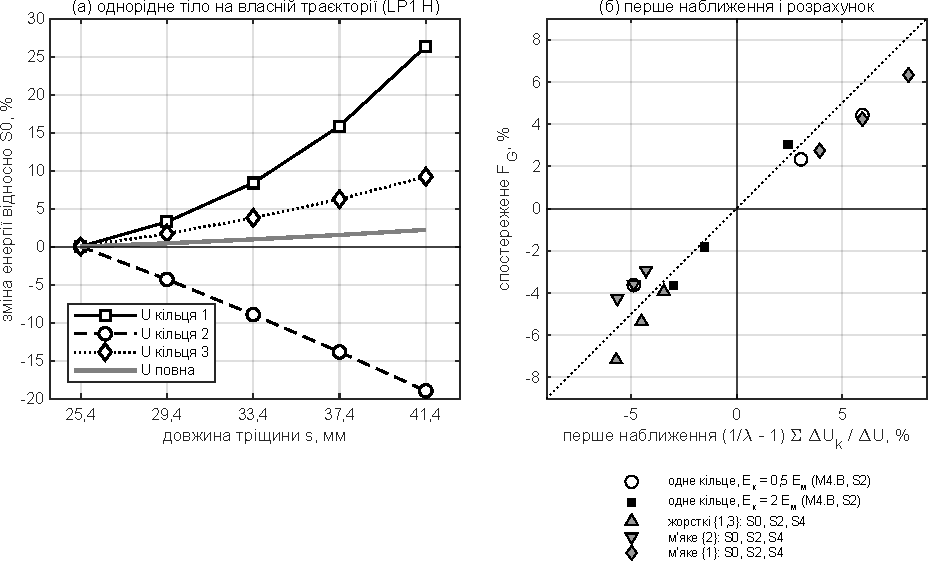
\includegraphics[width=\textwidth]{figures/G1_5_energii_kilets_UA.pdf}
 \caption{Зміна енергії в областях кілець уздовж однорідної траєкторії (а); зіставлення оцінки першого порядку та обчислених енергетичних контрастів (б). Частина архітектурних порівнянь виконана на різних власних траєкторіях.}
 \label{fig:ring-energy-evolution}
\end{figure}

Енергія в області кільця 2 монотонно зменшується на досліджених дискретних станах, тоді як в областях кілець 1 і 3 зростає. Це відповідає і змінам усереднених головних напружень: у кільці 2 модуль меншого головного напруження зменшується приблизно від $4{,}04$ до $3{,}50$ в одиницях $10^{-4}$ МПа, у кільці 1 збільшується розтягальна складова, у кільці 3 --- стискальна. Таким чином, відмінність полягає у характері перерозподілу енергії при рості тріщини, а не просто в наявності стиску.

\subsection{Кількісна перевірка оцінки першого порядку}

Для S2 застосуємо центральну різницю між S1 і S3:
\begin{equation}
 b_k^{\mathrm{FD}}=
 \frac{\mathcal W_k^{\mathrm H}(S3)-\mathcal W_k^{\mathrm H}(S1)}
 {\mathcal W_{\mathrm H}(S3)-\mathcal W_{\mathrm H}(S1)}.
 \label{eq:ring-b-fd}
\end{equation}
Інтервал довжини 8 мм скорочується у відношенні. Отримуємо $b_1=0{,}05959$, $b_2=-0{,}04872$, $b_3=0{,}03050$. Зіставимо $\eta_k b_k$ із результатами прямих розрахунків одиночних кілець.

\begin{table}[htbp]
 \centering
 \caption{Оцінка першого порядку та прямі розрахунки для одиночних кілець на S2, \%}
 \label{tab:ring-first}
 \begin{tabular}{rrrrr}
 \toprule
 & \multicolumn{2}{c}{$\lambda=0{,}5$} & \multicolumn{2}{c}{$\lambda=2$}\\
 \cmidrule(lr){2-3}\cmidrule(lr){4-5}
 Кільце & Оцінка & Розрахунок & Оцінка & Розрахунок\\
 \midrule
 1 & $+5,96$ & $+4,43$ & $-2,98$ & $-3,65$\\
 2 & $-4,87$ & $-3,63$ & $+2,44$ & $+3,04$\\
 3 & $+3,05$ & $+2,33$ & $-1,52$ & $-1,82$\\
 \bottomrule
 \end{tabular}
\end{table}

Знаки збігаються для всіх шести одиночних випадків. Для м'яких кілець оцінка завищує модуль ефекту, для жорстких --- занижує. Зіставлення з другою зовнішньою сіткою дає майже такі самі відношення обчисленого ефекту до оцінки. Додатково за збереженими однорідними станами виконано односторонні різниці на S0 та S4 і центральну на S2 для трьох вибраних архітектур. При S0 геометрія спільна; при S2 і S4 обчислений повний контраст містить також вплив різниці траєкторій. У сумі знаки збіглися в 21 із 21 пов'язаного порівняння (12 одиночних на двох сітках та 9 архітектурних). Це не 21 незалежне статистичне випробування.

Для м'яких архітектур і одиночних кілець відношення розрахунку до оцінки становить приблизно 0,68--0,78, для жорстких --- 1,14--1,26. Відхилення від оцінки сягають 14--32\,\% від її модуля. Це спостережені розбіжності за скінченного контрасту та різницевого наближення похідних; їх не можна ідентифікувати як виміряний член саме другого порядку. Для такого висновку потрібна серія малих контрастів і окрема перевірка похідної форми. Більш того, пізніші прямі перехресні розрахунки S4 не підтвердили наперед задані інтервали оцінки для stiff13 та soft1 (див. наступний розділ). Тому оцінка першого порядку пояснює знакову тенденцію, але не є універсальним кількісним предиктором.

\subsection{Просторова карта чутливості}

Вираз~\eqref{eq:ring-first-G} допускає просторове узагальнення. Для малої зміни матеріальної податливості $\eta(\boldsymbol x)$ в області, яка не перетинає тріщину чи її віртуальний приріст, введемо
\begin{equation}
 \iota(\boldsymbol x)=
 \frac{\partial_s w_{\mathrm H}(\boldsymbol x)}
 {\partial_s\mathcal W_{\mathrm H}},\qquad
 F_G^{(1)}=\int_\Omega\eta(\boldsymbol x)\iota(\boldsymbol x)
 \,\mathrm d\Omega .
 \label{eq:ring-influence}
\end{equation}
Густина $\iota$ має розмірність мм$^{-2}$. Її від'ємне значення означає екранувальну тенденцію при малому пом'якшенні відповідної області, додатне --- тенденцію підсилення. Це поле чутливості, а не густина енергії.

\begin{figure}[htbp]
 \centering
 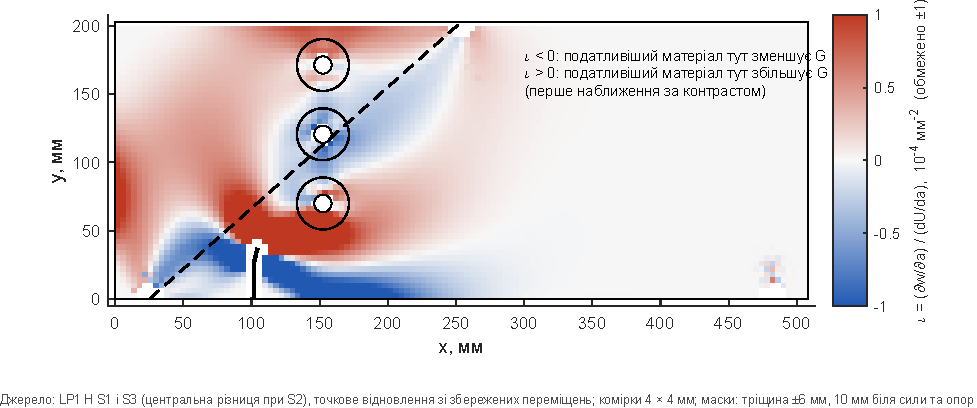
\includegraphics[width=\textwidth]{figures/G1_4_karta_vplyvu_UA.pdf}
 \caption{Різницеве наближення густини чутливості $\iota$ на S2 за однорідними полями S1 та S3. Масковано окіл тріщини й точки закріплення та навантаження; шкалу обмежено $\pm10^{-4}$ мм$^{-2}$.}
 \label{fig:ring-influence}
\end{figure}

Карту отримано точковим відновленням полів S1 та S3 на спільній координатній сітці з кроком 1 мм та усередненням по комірках 4 на 4 мм. Тріщину і зони по 10 мм навколо опор та сили виключено; біля тріщини ширина маски становить 6 мм з кожного боку. Інтегрування карти по кільцях дає приблизно 0,0606, $-0{,}0487$ та 0,0296, що відрізняється від~\eqref{eq:ring-b-fd} не більше ніж приблизно на 3\,\%. Різниця відображає просторове усереднення, маскування і різну дискретизацію станів; карта не є сертифікованою похідною.

Від'ємна область на боці сили охоплює кільце 2. Уздовж вертикальної лінії центрів кілець від'ємна смуга займає приблизно $82<y<158$ мм; кільце 2 повністю лежить у цьому інтервалі за висотою, кільця 1 і 3 зачеплені краями. Це пояснює знаки інтегральних чутливостей. На боці опори картина інша, а поблизу тріщини істотним є її власне ближнє поле. Необхідно уникати тлумачення всієї прямої опора--сила як єдиного силового стрижня.

\section{Вибір архітектур і межі фізичного пояснення}
\label{sec:ring-summary}

Проведене дослідження дозволило встановити, що розташування однакових за площею неоднорідностей змінює як знак, так і величину прямого енергетичного ефекту. Для пояснення протилежної ролі кільця 2 найбільш змістовним є не знак напруження, а енергетична чутливість до зміни геометрії тріщини. Її різницеве наближення відтворює знаки ефектів і дає правильний порядок величини. При цьому гіпотезу про розвантаження діагональної області передачі стискальних напружень підтверджено лише частково. Для виділення саме цього механізму необхідні контрольовані зміни положення сили, опор або кільця при збереженні інших параметрів. Такого розрахункового експерименту не виконано.

Для подальшої побудови власних траєкторій вибрано три архітектури: stiff13 --- жорсткі кільця 1 і 3 з найбільшим обчисленим екрануванням у серії S2; soft2 --- м'яке кільце 2 з від'ємним енергетичним ефектом і відносно малим напрямним ефектом; soft1 --- м'яке кільце 1 з підсиленням рушійної сили й істотним напрямним ефектом протилежного знака. Однорідна конфігурація H є опорною. Вибір забезпечує різні поєднання енергетичного та напрямного ефектів, а не три варіанти одного й того самого механізму.

Результат для soft2 на фіксованій S2 розрізняється за обома критеріями саме в цій серії. Це не гарантує консервативного розрізнення повного ефекту на наступних власних геометріях. Після незалежного розвитку тріщини прямий ефект матеріалу вже не збігається з повним ефектом, оскільки матеріал змінює також геометрію. Для розмежування цих двох впливів необхідні перехресні розрахунки. Їм присвячено наступний розділ.
